\documentclass{beamer}

\usefonttheme{professionalfonts} % using non standard fonts for beamer
\usefonttheme{serif} % default family is serif

\usepackage{hyperref}
%\usepackage{minted}
\usepackage{animate}
\usepackage{graphicx}
\def\Put(#1,#2)#3{\leavevmode\makebox(0,0){\put(#1,#2){#3}}}
\usepackage{colortbl}
\usepackage{tikz}
\usepackage{amssymb}
\usepackage{enumerate}
\usepackage{arydshln}
\usepackage{algorithm}
\usepackage{algpseudocode}

\colorlet{lightred}{red!25}
\colorlet{lightgreen}{green!25}
\beamertemplatenavigationsymbolsempty

\newcommand\blfootnote[1]{%
  \begingroup
  \renewcommand\thefootnote{}\footnote{#1}%
  \addtocounter{footnote}{-1}%
  \endgroup
}

\makeatletter

%% Textclass specific LaTeX commands.
\newcommand\makebeamertitle{\frame{\maketitle}}%
\AtBeginDocument{%
  \let\origtableofcontents=\tableofcontents
  \def\tableofcontents{\@ifnextchar[{\origtableofcontents}{\gobbletableofcontents}}
  \def\gobbletableofcontents#1{\origtableofcontents}
}
%% User specified LaTeX commands.
\usetheme{Malmoe}
\useoutertheme{infolines}
\addtobeamertemplate{headline}{}{\vskip2pt}
\setbeamercovered{transparent}

\makeatother

%%%%%%%%%%%%%%%%%%%%%%%%%%%%%%%%%%%%%%
%% Main document
%%%%%%%%%%%%%%%%%%%%%%%%%%%%%%%%%%%%%%
\begin{document}
\title[PFLOCK report]{PFLOCK Report}
\author[AC]{Andres Calderon}
\institute[Spring'20]{University of California, Riverside}
\makebeamertitle
\newif\iflattersubsect

\AtBeginSection[] {
    \begin{frame}<beamer>
    \frametitle{Outline} 
    \tableofcontents[currentsection]  
    \end{frame}
    \lattersubsectfalse
}

\AtBeginSubsection[] {
    \begin{frame}<beamer>
    \frametitle{Outline} 
    \tableofcontents[currentsubsection]  
    \end{frame}
}

\begin{frame}{Ensuring all data is in each partition}
  \begin{itemize}
    \item Points are partitioned according to $\varepsilon$ before finding pairs (pairs of points lying $\varepsilon$ each other).    
  \end{itemize}
\end{frame}

\begin{frame}
  \centering
  \vspace{-7pt}
  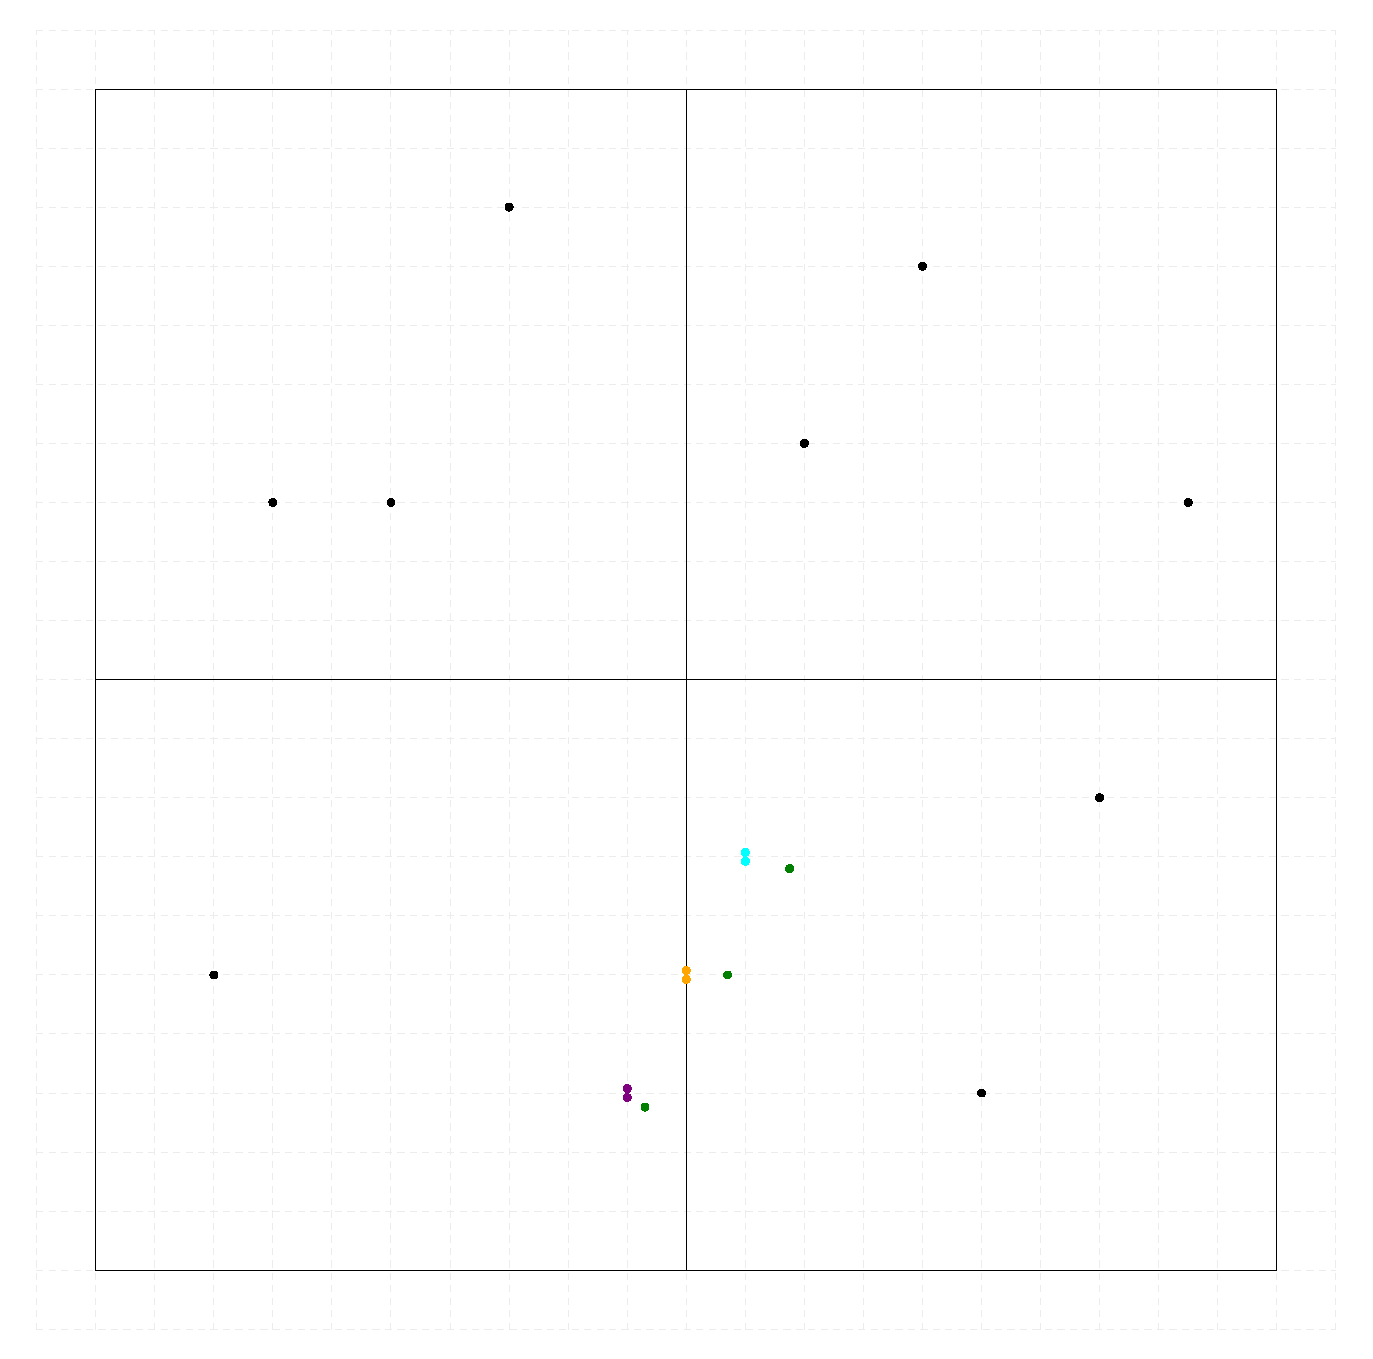
\includegraphics[page=1, scale=0.4]{figures/centers}
\end{frame}
\begin{frame}
  \centering
  \vspace{-7pt}
  \includegraphics[page=2, scale=0.4]{figures/centers}
\end{frame}
\begin{frame}
  \centering
  \vspace{-7pt}
  \includegraphics[page=3, scale=0.4]{figures/centers}
\end{frame}
\begin{frame}
  \centering
  \vspace{-7pt}
  \includegraphics[page=4, scale=0.4]{figures/centers}
\end{frame}
\begin{frame}
  \centering
  \vspace{-6pt}
  \includegraphics[page=5, scale=0.35]{figures/centers}
\end{frame}
\begin{frame}
  \centering
  \vspace{-6pt}
  \includegraphics[page=6, scale=0.35]{figures/centers}
\end{frame}
\begin{frame}
  \centering
  \vspace{-6pt}
  \includegraphics[page=7, scale=0.35]{figures/centers}
\end{frame}
\begin{frame}
  \centering
  \vspace{-6pt}
  \includegraphics[page=8, scale=0.35]{figures/centers}
\end{frame}

\begin{frame}{What's next}
    \begin{itemize}
        \item test.
    \end{itemize}
\end{frame}

\end{document}

